\chapter{Ensemble Learning}
\label{chapter:Ensemble Learning}

Ensemble Learning is a class of supervised learning algorithms that use multiple models instead of a single one to obtain better predictions. A common problem with classifiers is that not all classifiers are suited for all kinds of problems. Ensembles of classifiers involve combinining multiple classifiers to construct an expectantly better classifier. The performance of an ensemble is not guaranteed to be better than the individual classifiers, but depending on the problem, an ensemble usually outperforms its constituent classifiers by a fair margin. But like almost all machine learning methods, a generalization cannot be made and it depends a lot on the problem at hand. Using ensemble learning requires performing more computation, but yields better results when the classifiers are not similar to each other.

\section{Bagging}
Bagging, also referred to as Bootstrap Aggregation, is one of the most basic forms of ensemble learning. Given a training dataset $D$ containing $N$ samples, each sample having $D$ different features, the aim of bagging is to combine $M$ classifiers, each trained using a different subset of the main data, such that every classifier learns about a different structure of the input data. When the outputs from all the constituent classifiers are combined, the final output is expected to be better than the individual predictions. Bagging requires that the entire system should not be stable, so that when the training data changes by even small amounts, the resulting classifiers are different \cite{quinlan1996bagging}. A consequence of this was also presented in \cite{breiman1996bagging}, where it was noted that for unstable classifiers, bagging introduces improvements in the net classifier accuracy. On the other hand, if the underlying classifiers are already strong and stable, the performance may degrade a little \cite{breiman1996bagging}. Bagging is often known as the less risky approach, in that there is a high chance that using bagging improves the performance of the classifier.\\

To train different classifiers on a different subset of the data, the training data is either split on the number of samples, or on the number of features. In the first case, $N' (< N)$ samples are picked with replacement, and each time a new classifier is trained using the new dataset. Since the data points are picked with replacement, some of the data points may be common to some classifiers. In the second case, every new classifier is trained using $M' (< M)$ features with replacement. Whenever the ensemble is required to make a prediction on a new sample, a majority vote from all the constituent classifiers is taken, which becomes the final output of the ensemble.

\section{Boosting}
The original hypothesis behind Boosting was the notion that a set of weak learners can be trained to form a strong learner \cite{kearns1988thoughts}. Boosting aims to build an ensemble of classifiers by iteratively training weak classifiers on a distribution, and then finally putting them all together to build a strong classifier. In the training phase, the classifiers are trained one by one. Each training instance is assigned a numeric weight, which is the same for all samples in the beginning. After the first classifier has been trained, the weights for the points which were misclassified are increased, and the resulting input data (along with the modified weight values) is fed to the second classifier. This process continues until the last classifier has been trained. This way, each classifier has an incentive to focus more on classifying correctly those points which the previous classifier classified incorrectly.\\

Each classifier's performance is maintained in a vector (usually named $\alpha$). Whenever a new point has to be classified, the individual predictions are obtained from the constituent classifiers, and a weighted sum (from the $\alpha$ values) is taken across all the classifiers to obtain the final prediction. One of the very popular Boosting techniques is Adaptive Boosting, originally presented in \cite{freund1995desicion}. The main aim of Boosting is to build a strong classifier from a set of weak classifiers. To that effect, even classifiers only slightly better than random are considered useful, because in the final predictions, they will still contribute positively to the aggregate prediction by behaving like their inverses because of having negative coefficients in the final linear combination of classifiers.\\

The algorithm used to train a model over a dataset is the following.

\begin{enumerate}
    \item{Initialize the sample weights $w_n = 1/N$, for $n = 1, 2, ..., N$}
    \item{
    For $m = 1, 2, ..., M$:
    \begin{itemize}
        \item{Train a classifier $\mathbf{y_m(x)}$ on the training data using the sample weights $\mathbf{w}$}
        \item{Calculate $$\epsilon_m = \frac{\displaystyle \sum_{n = 1}^{N} w_n I_n}{\displaystyle \sum_{n = 1}^{N} w_n}$$ where $I(y_m(x_n) \neq y_n)$ is the indicator function and equals 1 when the predicted label $y_m(x_n) \neq$ the actual label $y_n$, and 0 otherwise}
        \item{Set $$\alpha_m = \log(\frac{1 - \epsilon_m}{\epsilon_m})$$}
        \item{Update $\mathbf{w}$ using $$w_n := w_n \exp(\alpha_m I(y_m(x_n) \neq y_n))$$}
    \end{itemize}
    }
\end{enumerate}

After all the models have been trained, the prediction for an instance $x_n$ is obtained by calculating $$sign(\displaystyle \sum_{m = 1}^{M} \alpha_m y_m(x_n))$$

\section{Stacking}
Stacking, also called Stacked Generalization was first introduced in \cite{wolpert1992stacked}, and obtains predictions by a two step process. It is assumed that there exists a training input matrix that has $N$ rows for $D$ samples, and $D$ columns for $D$ features. In the first step, $M$ distinct classifiers are trained on the training data. After the classifiers have been trained, a new dataset of $N$ rows and $M$ columns is generated, each column being populated by predictions for each of the $M$ classifiers. This new dataset forms the training data for a second level classifier, from which the final prediction is obtained. The process for prediction from a Stacking ensemble follows a similar path. Given a sample $x_n$ of the form $[(\mathbf{x}_{n, 1}, \mathbf{x}_{n, 2}, ... \mathbf{x}_{n, D})]$, it is first run through the $M$ classifiers to obtain $M$ predictions $(y_m)$ for $m = 1, 2, ..., M$. These values are then fed to the second level classifier, which yields the final label.\\

\begin{figure}
    \centering
    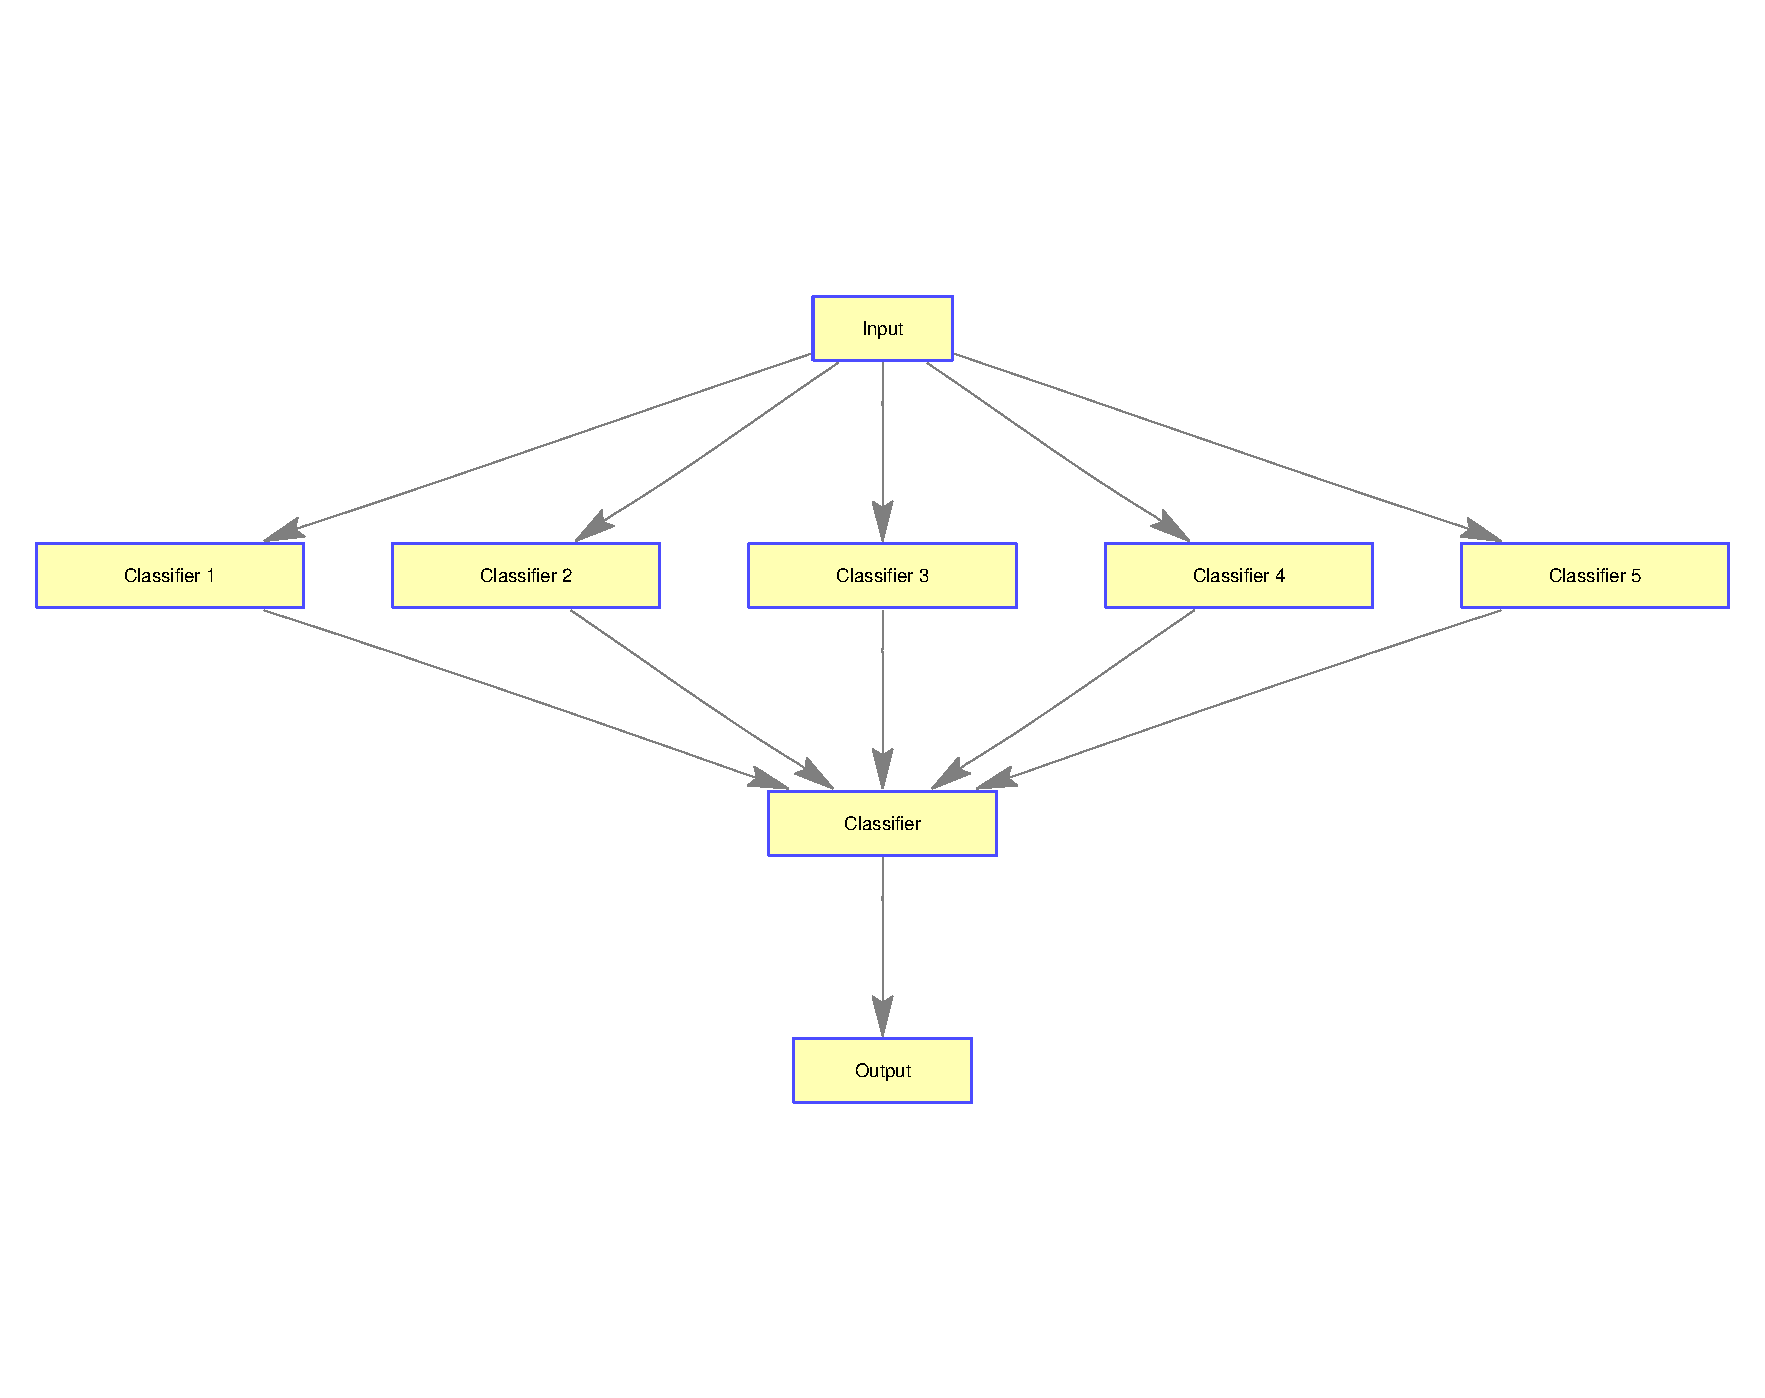
\includegraphics[width=0.8\textwidth]{stacking_flow.eps}
    \caption{Stacking}
    \label{fig:stacking_flow}
\end{figure}

Figure~\ref{fig:stacking_flow} illustrates how stacking works when there are 5 classifiers at the first level. The node ``Input'' refers to the sample $x_n$ for which the prediction is to be made. It is fed to each classifier, and the resulting predictions from the classifiers form an $M$ dimensional vector, which is then fed to the main classifier at the second level, which then gives the final label. Two of the most common schemes for training classifiers at the first level include bootstrapping (training different classifiers using different subsets of data) and feature sampling (using different features as inputs for different classifiers). Stacking is one of the best ensemble learning methods that has proven to be successful in a number of works, as well as in the real world. The study done in \cite{dvzeroski2004combining} experimented with a number of datasets to compare stacking against multiple schemes for combining classifiers, to discover that a stacking ensemble performs much better than when classifiers are combined using the \emph{voting} or \emph{select-best} schemes. The nature of inputs for the second level classifier were studied in \cite{ting2011issues}. This work concluded that much better results can be obtained if the confidence values from the first level classifiers are included in the input for the higher level model. Stacking was also employed by the winning team at the Netflix prize \cite{koren2009bellkor}, in which the solution included meta features as inputs (number of users and number of movie ratings) in addition to using the normal feature vectors.
